\documentclass{standalone}
% \documentclass{article}

\usepackage{tikz}
\usetikzlibrary{calc}

\begin{document}

    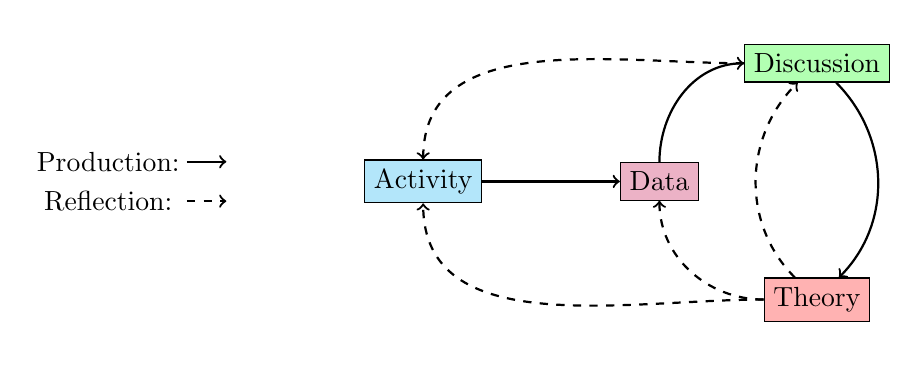
\begin{tikzpicture}
        % Nodes
        \node (activity) at (0,0) [fill=cyan!30, draw] {Activity};
        \node (data) at ($(activity) + (3,0)$) [fill=purple!30, draw] {Data};
        \node (discussion) at ($(data) + (2,1.5)$) [fill=green!30, draw] {Discussion};
        \node (theory) at ($(data) + (2,-1.5)$) [fill=red!30, draw] {Theory};

        % Creative arrows
        \draw [thick, ->] (activity) -- (data);
        \draw [thick, ->] (data) edge[out=90, in=180] (discussion);
        \draw [thick, ->] (discussion) edge[out=-45, in=45] (theory);

        % Reflective arrows
        \draw [thick, ->, dashed] (theory) edge[out=180, in=-90] (data);
        \draw [thick, ->, dashed] (theory) edge[out=180, in=-90] (activity);
        \draw [thick, ->, dashed] (discussion) edge[out=180, in=90] (activity);
        \draw [thick, ->, dashed] (theory) edge[out=135, in=-135] (discussion);

        % Key
        \draw [thick, ->] ($(activity) + (-3,.25)$) -- ($(activity) + (-2.5,.25)$);
        \node at ($(activity) + (-4, .25)$) {Production:};
        \draw [thick, ->, dashed] ($(activity) + (-3,-.25)$) -- ($(activity) +
        (-2.5,-.25)$);
        \node at ($(activity) + (-4, -.25)$) {Reflection:};

    \end{tikzpicture}

\end{document}
